\documentclass[xetex]{beamer}

\usepackage{fontspec}
\usepackage[autostyle]{csquotes}
\usepackage{hyperref}
\usepackage{color}

\title{Un Pinguino piccolo piccolo}
\subtitle{Linux nei sistemi embedded}
\author{Luca Ceresoli}
\date{Linux Day --- BgLUG --- Sabato 24 ottobre 2015}

\AtBeginSection[]
{
  \begin{frame}
    \frametitle{Table of Contents}
    \tableofcontents[currentsection]
  \end{frame}
}

\begin{document}

\maketitle

\section{Introduzione}

\begin{frame}
  \frametitle{Che cosa è un sistema embedded}

  \blockquote{In elettronica e informatica, con il termine sistema
    embedded (letteralmente immerso o {\color{red} incorporato}) si
    identificano genericamente tutti quei {\color{violet} sistemi
      elettronici di elaborazione a microprocessore} progettati
    appositamente per una determinata applicazione
    ({\color{blue}special purpose}) ovvero non riprogrammabili
    dall'utente per altri scopi, spesso con una piattaforma
    {\color[rgb]{0,0.5,0} hardware ad hoc}, integrati nel sistema che
    controllano ed in grado di gestirne tutte o parte delle
    funzionalità richieste.}

  (Fonte:
  \url{https://it.wikipedia.org/w/index.php?title=Sistema_embedded&oldid=73160266})
\end{frame}

  \begin{frame}{}
    \huge
    \begin{center}
      Esempi...
    \end{center}
  \end{frame}

\begin{frame}
  \frametitle{Router ADSL}
  \begin{center}
    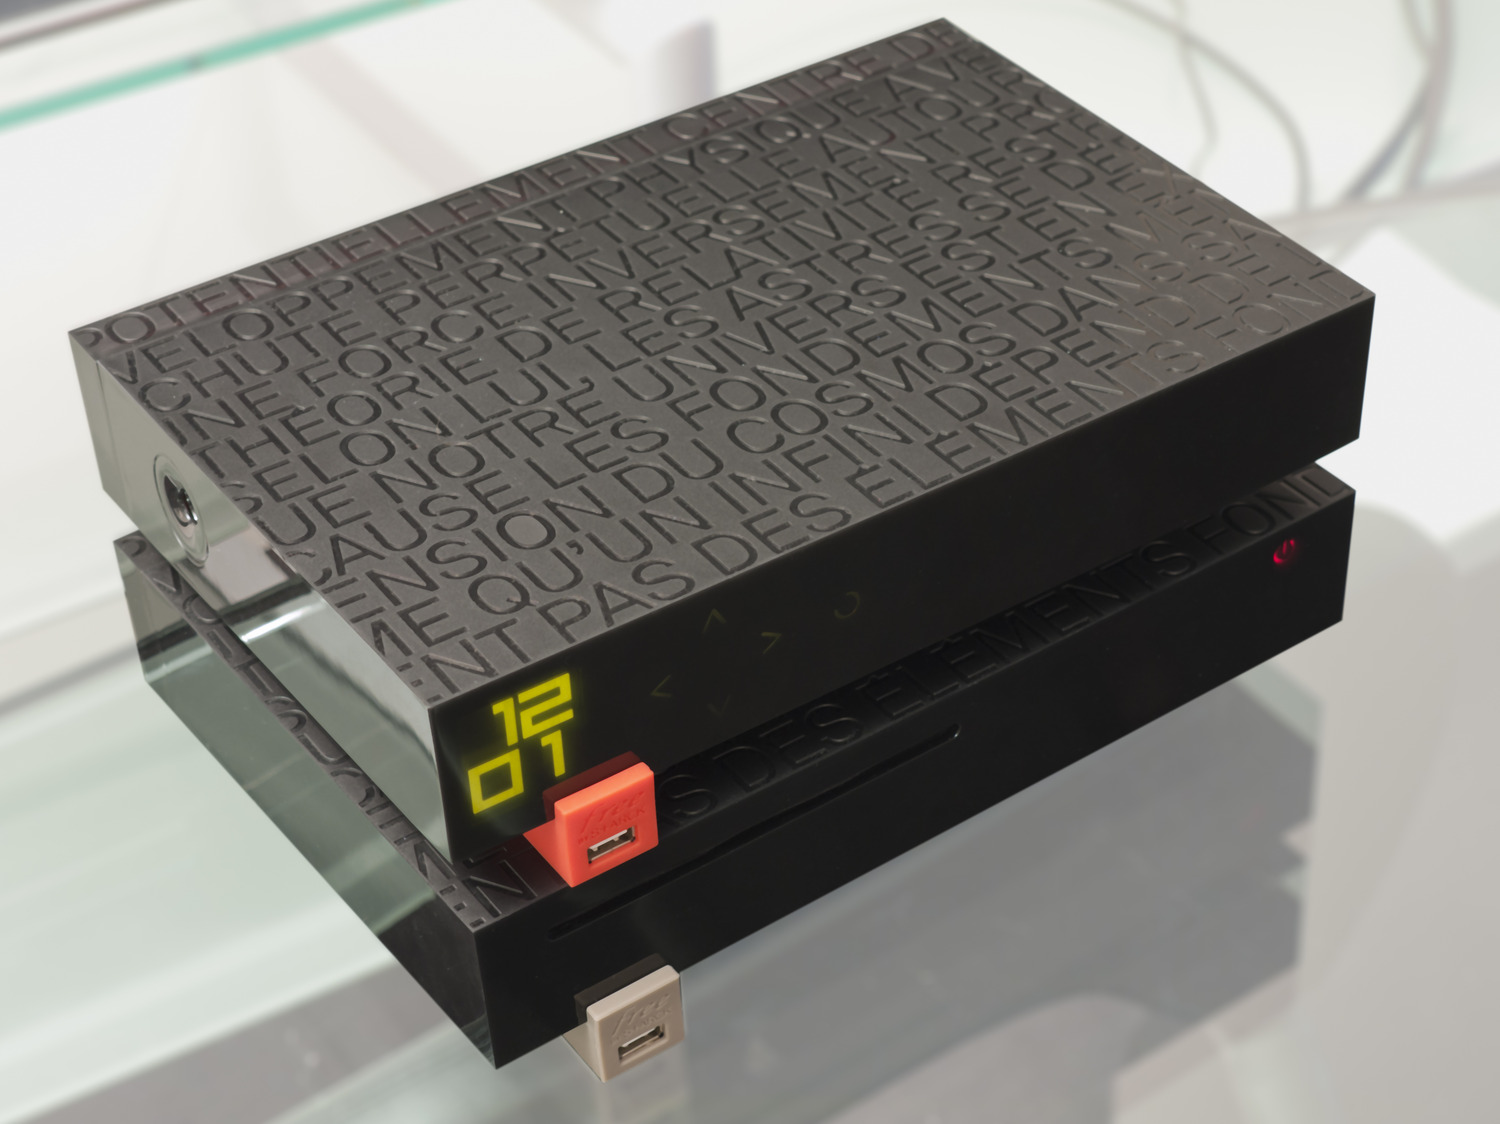
\includegraphics[width=0.7\textwidth]{images/freebox.jpg}
  \end{center}
\end{frame}

\begin{frame}
\frametitle{Televisione}
  \begin{center}
    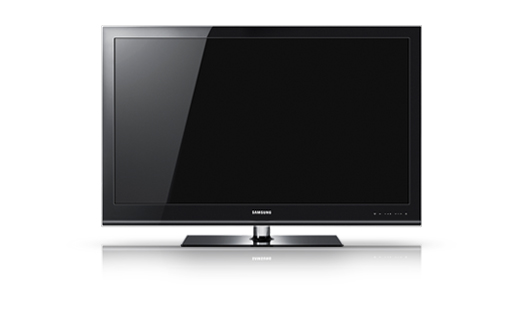
\includegraphics[width=0.7\textwidth]{images/television.jpg}
  \end{center}
\end{frame}

\begin{frame}
\frametitle{Terminale POS}
  \begin{center}
    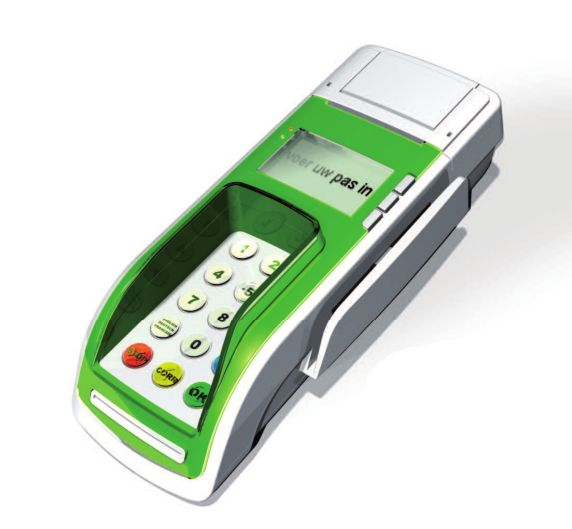
\includegraphics[width=0.7\textwidth]{images/point-of-sale.jpg}
  \end{center}
\end{frame}

\begin{frame}
\frametitle{Tagliatrice laser}
  \begin{center}
    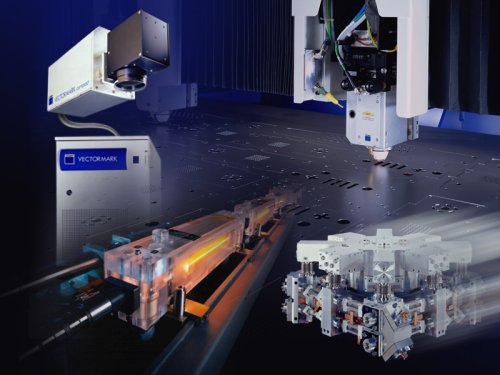
\includegraphics[width=0.7\textwidth]{images/laser-cutting-machine.jpg}
  \end{center}
\end{frame}

\begin{frame}
\frametitle{Macchina per viticultura}
  \begin{center}
    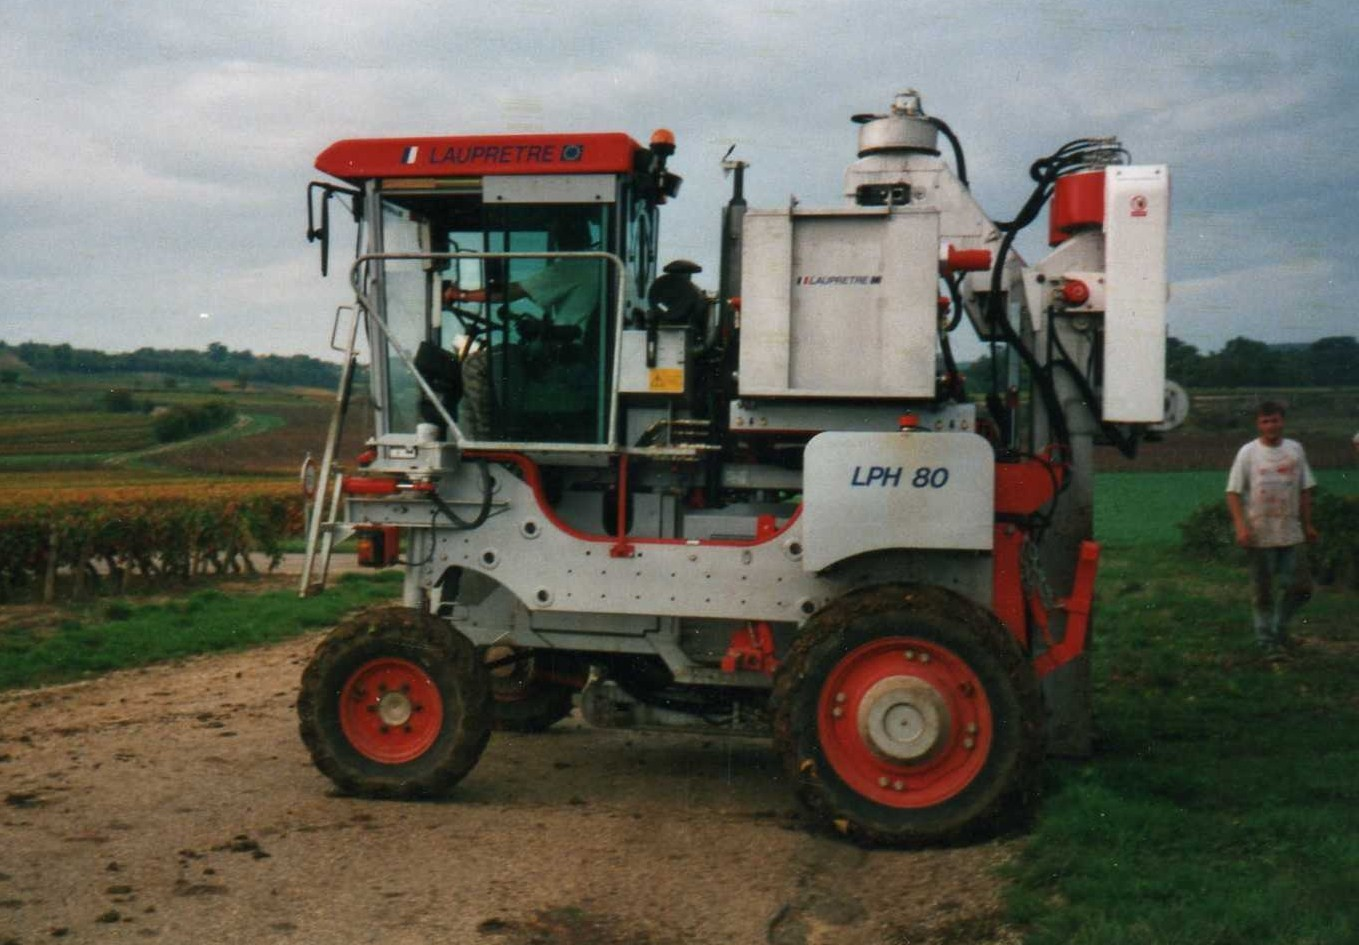
\includegraphics[width=0.7\textwidth]{images/viticulture-machine.jpg}
  \end{center}
\end{frame}

\section{Sfida \#1: Risorse disponibili}

\section{Sfida \#2: Cross-compilazione}

\section{Sfida \#3: Nessuno standard}

\section{Sfida \#4: Comporre un puzzle}

\end{document}
